\documentclass[tikz,border=5pt]{standalone}
\usepackage[T1]{fontenc}
\usepackage{lmodern,amsmath,amssymb}
\usetikzlibrary{arrows.meta,calc,positioning,fit,backgrounds,shapes.geometric,matrix,decorations.pathreplacing,patterns}
\definecolor{ink}{gray}{0.08}
\definecolor{wash}{gray}{0.965}
\definecolor{soft}{gray}{0.45}
\tikzset{box/.style={draw=ink,line width=.65pt,fill=white,align=center,inner sep=4pt,outer sep=0pt,font=\small},flow/.style={draw=ink,line width=.65pt,-{Latex[length=1.8mm,width=1.3mm]},rounded corners=2pt},annotation/.style={font=\scriptsize,text=soft,align=center},groupbox/.style={draw=soft,dashed,line width=.45pt,fill=wash}}
\begin{document}
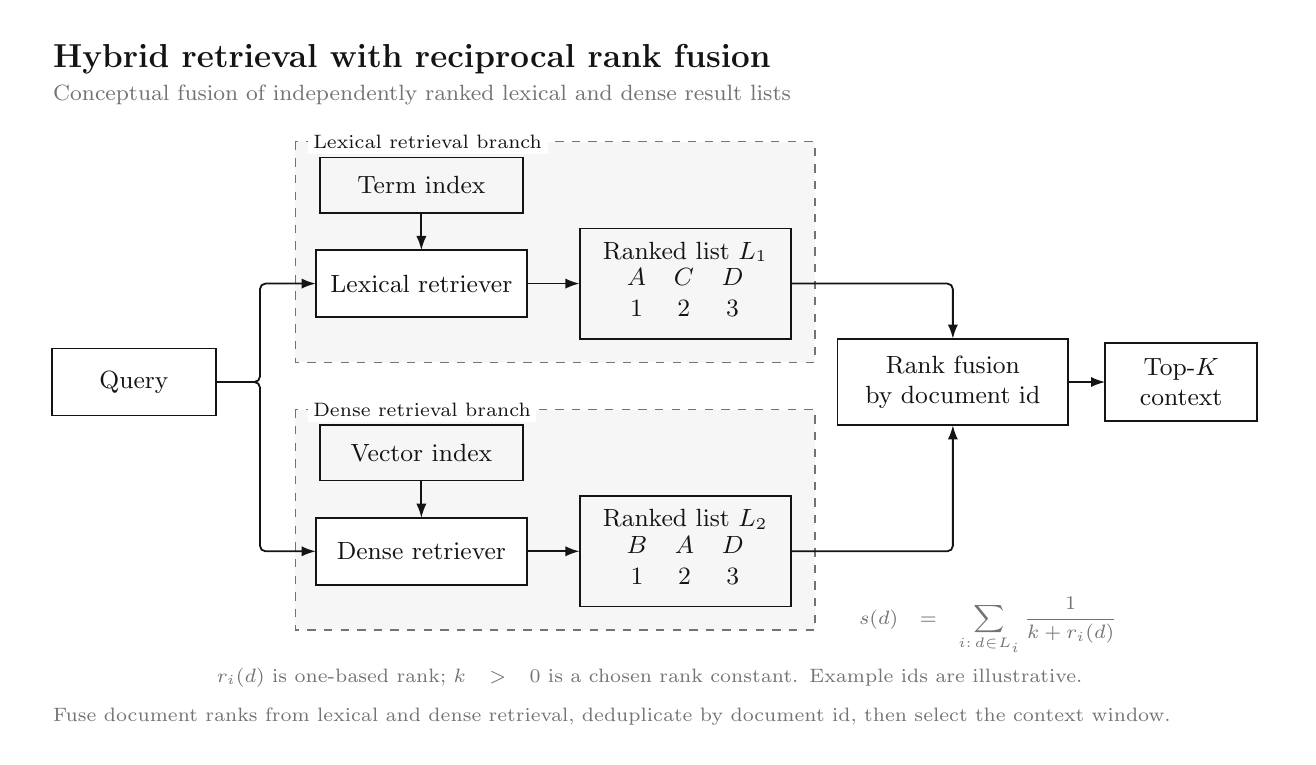
\begin{tikzpicture}[x=1cm,y=-1cm,font=\rmfamily,text=ink]

\path[use as bounding box] (0,0) rectangle (16,9);
\node[anchor=west,font=\large\bfseries] at (.2,.4) {Hybrid retrieval with reciprocal rank fusion};
\node[anchor=west,font=\footnotesize,text=soft] at (.2,.85) {Conceptual fusion of independently ranked lexical and dense result lists};
\begin{pgfonlayer}{background}
\draw[groupbox] (3.4,1.45) rectangle (10.0,4.25);
\node[anchor=west,font=\scriptsize,fill=white,inner sep=2pt] at (3.55,1.45) {Lexical retrieval branch};
\draw[groupbox] (3.4,4.85) rectangle (10.0,7.6499999999999995);
\node[anchor=west,font=\scriptsize,fill=white,inner sep=2pt] at (3.55,4.85) {Dense retrieval branch};
\end{pgfonlayer}
\node[box,minimum width=2.05cm,minimum height=0.85cm,text width=1.7999999999999998cm] (q) at (1.35,4.5) {Query};
\node[box,fill=wash,minimum width=2.55cm,minimum height=0.7cm,text width=2.3cm] (terms) at (5.0,2.0) {Term index};
\node[box,minimum width=2.65cm,minimum height=0.85cm,text width=2.4cm] (lexical) at (5.0,3.25) {Lexical retriever};
\node[box,fill=wash,minimum width=2.65cm,minimum height=1.4cm,text width=2.4cm] (list1) at (8.35,3.25) {Ranked list $L_1$\\$\begin{array}{ccc} A&C&D\\1&2&3\end{array}$};
\node[box,fill=wash,minimum width=2.55cm,minimum height=0.7cm,text width=2.3cm] (vectors) at (5.0,5.4) {Vector index};
\node[box,minimum width=2.65cm,minimum height=0.85cm,text width=2.4cm] (dense) at (5.0,6.65) {Dense retriever};
\node[box,fill=wash,minimum width=2.65cm,minimum height=1.4cm,text width=2.4cm] (list2) at (8.35,6.65) {Ranked list $L_2$\\$\begin{array}{ccc} B&A&D\\1&2&3\end{array}$};
\node[box,minimum width=2.9cm,minimum height=1.1cm,text width=2.65cm] (fusion) at (11.75,4.5) {Rank fusion\\by document id};
\node[box,minimum width=1.9cm,minimum height=1.0cm,text width=1.65cm] (context) at (14.65,4.5) {Top-$K$\\context};
\begin{pgfonlayer}{background}
\draw[flow] (q.east) -- (2.95,4.5) -- (2.95,3.25) -- (lexical.west);
\draw[flow] (q.east) -- (2.95,4.5) -- (2.95,6.65) -- (dense.west);
\draw[flow] (terms.south) -- (lexical.north);
\draw[flow] (vectors.south) -- (dense.north);
\draw[flow] (lexical.east) -- (list1.west);
\draw[flow] (dense.east) -- (list2.west);
\draw[flow] (list1.east) -- (11.75,3.25) -- (fusion.north);
\draw[flow] (list2.east) -- (11.75,6.65) -- (fusion.south);
\draw[flow] (fusion.east) -- (context.west);
\end{pgfonlayer}
\node[annotation,anchor=center,text width=6.0cm] at (12.2,7.6) {$s(d)=\displaystyle\sum_{i:\,d\in L_i}\frac{1}{k+r_i(d)}$};
\node[annotation,anchor=center,text width=14cm] at (7.9,8.25) {$r_i(d)$ is one-based rank; $k>0$ is a chosen rank constant. Example ids are illustrative.};
\node[anchor=west,align=left,font=\scriptsize,text=soft,text width=15.6cm] at (.2,8.75) {Fuse document ranks from lexical and dense retrieval, deduplicate by document id, then select the context window.};
\end{tikzpicture}
\end{document}
